\documentclass[journal]{IEEEtran}

\usepackage[T1]{fontenc}% optional T1 font encoding

\ifCLASSINFOpdf

\else

\fi

\usepackage{amsmath}

\interdisplaylinepenalty=250 %0

\usepackage{graphicx}
\usepackage{cite}
\usepackage{amsmath}

\begin{document}

\title{Report for the First Assignment of Reinforcement Learning Course, CISC 856, Fall 2019}


\author{Milad Khademi Nori (20187733), Azadeh Motamedi (20188887)}% <-this % stops a space

\maketitle

%\begin{abstract}
%\end{abstract}

%\begin{IEEEkeywords}
%Energy Harvesting Wireless Sensor Networks (EH-WSNs), Cluster Head (CH), Residual Energy (RE), Energy Harvesting Rate (EHR), Energy Harvesting (EH).
%\end{IEEEkeywords}

\IEEEpeerreviewmaketitle

%\section{Organization of This Report}
%This section, as the first section, explains how I organized my report. There are three sections to this report, other than the current one. In section II, we investigate the first policy for all three games, while section III studied the second policy. Finally, in section IV, we conclude all of the results.

\section{First Policy}
%his section of the report is intended for the first policy iteration algorithm. The followings are the answers to the corresponding questions.
\subsection{Prisoners' Dilemma}
(a) For the first game, namely the prisoners' dilemma, the policy of the player $j$ almost converges to $p^{j}= [p^{j}_{1}, p_{2}^{j}]=[0, 1]$, where $p^{j}_{1}$ and $p^{j}_{2}$ denote the probability of cooperation and defection. These number indicate that player $j$ (prisoner $j$) has the tendency not to cooperate. According to simulations, Figure \ref{Fig:firstPolFirstGame1} and \ref{Fig:firstPolFirstGame2} show the trajectory of policies that converge to the origin where indicates that prisoners are discouraged from cooperating. It is worth mentioning that the policy distribution at the beginning of iteration is shown by violet; it changes color gradually until it reaches the final point shown in red. %This convention is maintained throughout this report.
%We observe that for different initial policy distributions, there is a little possibility of converging to the $[1, 1]$


\begin{figure}[!h]
\centering
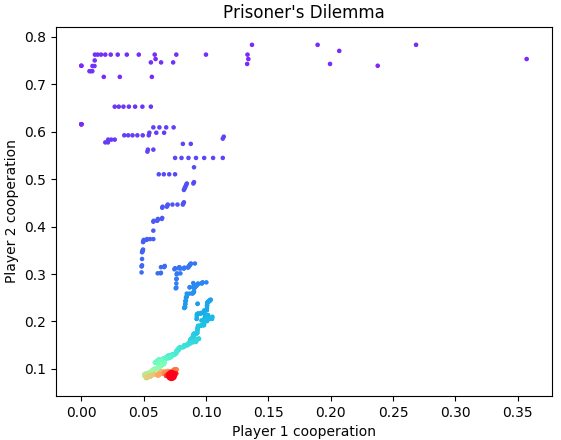
\includegraphics[scale=0.35]{figure/firstGameFirstPolicy4m.png}
\caption{Policy convergence trajectory of player 1 cooperation versus player 2 cooperation. Start point $(0.35, 0.75)$, end point $(0.07, 0.08)$}
\label{Fig:firstPolFirstGame1}
\end{figure}


\begin{figure}[!h]

\centering
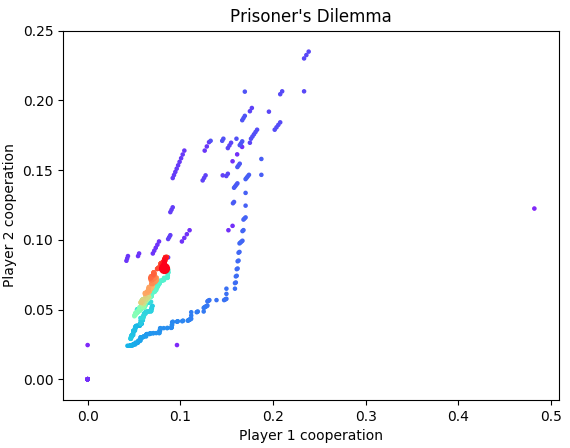
\includegraphics[scale=0.35]{figure/firstGameFirstPolicy3m.png}
\caption{Policy convergence trajectory of player 1 cooperation versus player 2 cooperation.
Start point $(0.48, 0.12)$, end point $(0.07, 0.07)$}
\label{Fig:firstPolFirstGame2}
\end{figure}

(b) No, the policy is not optimal (or Pareto optimal), it is a Nash equilibrium. Nash equilibrium is an outcome in which every player is doing the best he possibly can, given the other players' choices. Therefore, no player can benefit from unilaterally changing his choice. In this example if any player changes his choices he get $0$ as opposed to $1$ that he is currently receiving.

\subsection{Matching Pennies}
(a) The policy of the player $j$ almost gets close (does not meet) to $p^{j}= [p^{j}_{1}, p_{2}^{j}]=[0.5, 0.5]$, where $p^{j}_{1}$ and $p^{j}_{2}$ denote the probability of selecting head and tail. According to simulations, Figure \ref{Fig:secondPolFirstGame3} and \ref{Fig:secondPolFirstGame4} show the trajectory of policies that do not converge to the center $(0.5, 0.5)$ and circulates it \cite{the}. Players try to select each side of the coin with equal probability which has the most uncertainty for the opponent.


\begin{figure}[!t]
\centering
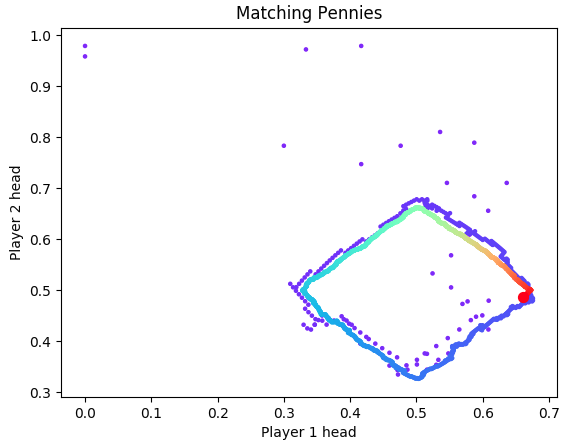
\includegraphics[scale=0.35]{figure/secondGameFirstPolicy2m.png}
\caption{Policy convergence trajectory of player 1 head versus player 2 head. Start point $(0.91, 0.92)$, end point $(0.53, 0.62)$}
\label{Fig:secondPolFirstGame3}
\end{figure}

\begin{figure}[!t]

\centering
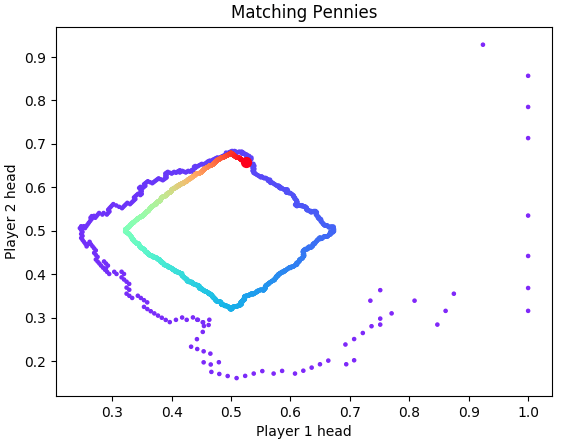
\includegraphics[scale=0.35]{figure/secondGameFirstPolicy4m.png}
\caption{Policy convergence trajectory of player 1 head versus player 2 head.
Start point $(0.48, 0.12)$, end point $(0.07, 0.07)$}
\label{Fig:secondPolFirstGame4}
\end{figure}

(b) Yes, the policy is optimal (Pareto optimal) and it is a Nash equilibrium as well. In this example if any player changes his choices from $0.5$ to more or less, he would decrease the uncertainty of the opponent. Besides, this game is a zero-sum game (fair game) which implies that expectation of reward is 0 for both.

\begin{figure}[!t]
\centering
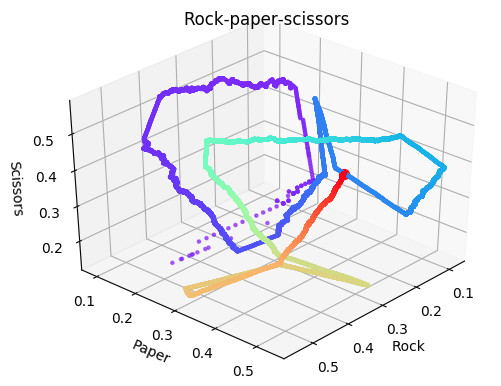
\includegraphics[scale=0.37]{figure/thirdGameFirstPolicy1m.png}
\caption{Policy convergence trajectory of the first player. Start point $(0.55, 0.3, 0.15)$, end point $(0.22, 0.40, 0.38)$}
\label{Fig:thirdPolFirstGame5}
\end{figure}

\begin{figure}[!t]

\centering
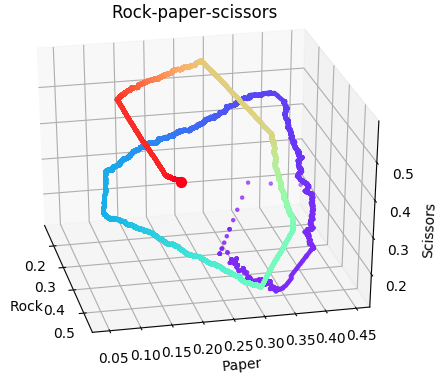
\includegraphics[scale=0.37]{figure/thirdGameFirstPolicy2m.png}
\caption{Policy convergence trajectory of the first player. Start point $(0.25, 0.45, 0.30)$, end point $(0.30, 0.25, 0.45)$}
\label{Fig:thirdPolFirstGame6}
\end{figure}
\subsection{Rock-paper-scissors}
(a) The policy of the player $j$ almost converges to $p^{j}= [p^{j}_{1}, p_{2}^{j}, p_{3}^{j}]=[1/3, 1/3, 1/3]$, where $p^{j}_{1}$, $p^{j}_{2}$, and $p^{j}_{3}$ denote the probability of selecting rock, paper, and scissors, respectively. According to simulations, Figure \ref{Fig:thirdPolFirstGame5} and \ref{Fig:thirdPolFirstGame6} show the trajectory of policies that gets close to the  $(0.33, 0.33, 0.33)$ and circulates \cite{the}. Players select each action with equal probability which has the most uncertainty for the opponent.

(b) Yes, the policy is optimal (Pareto optimal) and it is a Nash equilibrium as well. In this example if any player changes his choices from $0.33$ to more or less, he would decrease the uncertainty of the opponent.

\section{Second Policy} 
\subsection{Prisoners' Dilemma}

(c) This time with the new policy iteration algorithm, it has been observed that the algorithm converges to the origin considerably smoother because the appended term serves as a stabilizer; more precisely, when the first term spikes and pushes the policy value to increase, the second term (appended term) somehow damps the immediate changes and guides the policy toward the expected value. This term might have some downsides when the process is non-stationary that makes the policy less responsive to new environments. Figure \ref{Fig:secondPolFirstGame7} and \ref{Fig:secondPolFirstGame8} corroborates our expectations.


\begin{figure}[!t]
\centering
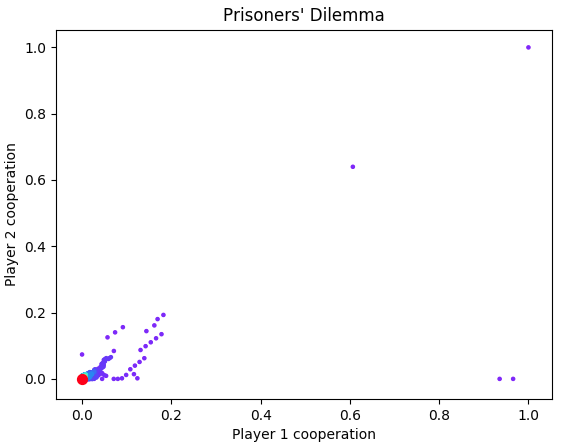
\includegraphics[scale=0.37]{figure/firstGameSecondPolicy3m.png}
\caption{Policy convergence trajectory of player 1 cooperation versus player 2 cooperation. Start point $(1, 1)$, end point $(0, 0)$}
\label{Fig:secondPolFirstGame7}
\end{figure}

\begin{figure}[!t]

\centering
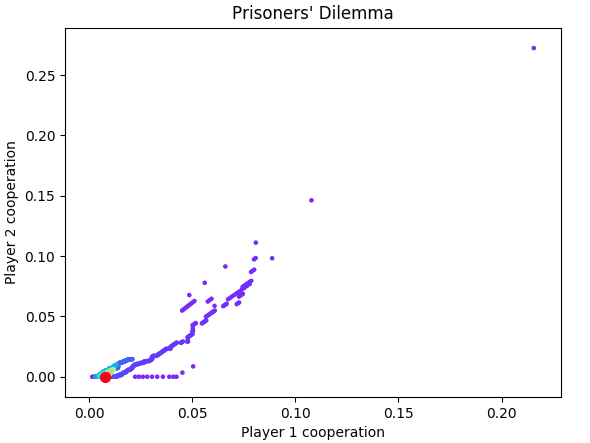
\includegraphics[scale=0.37]{figure/firstGameSecondPolicy4m.png}
\caption{Policy convergence trajectory of player 1 cooperation versus player 2 cooperation. Start point $(0.22, 0.26)$, end point $(0.01, 0)$}
\label{Fig:secondPolFirstGame8}
\end{figure}
(d) As mentioned before, it is not optimal since there is another point on which both players can receive more reward, but we can say it is a Nash equilibrium. 

(e) The value of the game is typically about $1.7$. The decimal part stems from the occasion when players have not yet been trapped in Nash equilibrium.

(f) Because the extra term helps to stabilize policy iteration; more precisely, when the first term bounces and pushes the policy value to fluctuate, the second term (added term) somehow hampers the instant changes and leads the policy toward the expected value.
\subsection{Matching Pennies}

(c) The new algorithm performs better for matching pennies game, gets closer to $(0.5, 0.5)$ point, and circulates it but still does not converge to it \cite{the} (shown in Figure \ref{Fig:secondPolSecondGame9} and \ref{Fig:secondPolSecondGame10}).


\begin{figure}[!t]
\centering
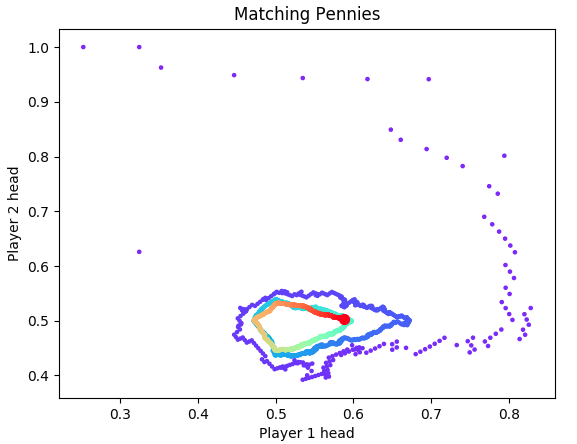
\includegraphics[scale=0.37]{figure/secondGameSecondPolicy1m.png}
\caption{Policy convergence trajectory of player 1 head versus player 2 head. Start point $(0.10, 1)$, end point $(0.59, 0.50)$}
\label{Fig:secondPolSecondGame9}
\end{figure}

\begin{figure}[!t]

\centering
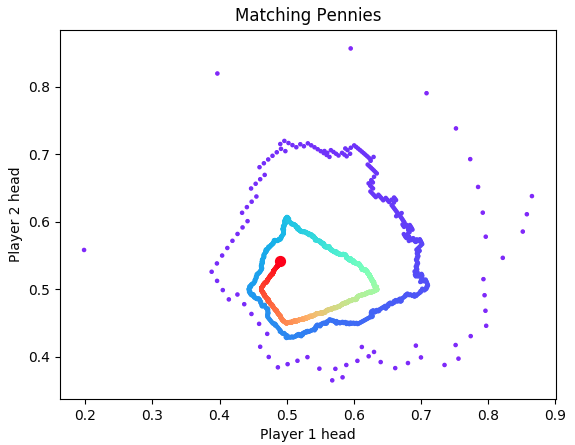
\includegraphics[scale=0.37]{figure/secondGameSecondPolicy2m.png}
\caption{Policy convergence trajectory of player 1 head versus player 2 head. Start point $(0.20, 0.56)$, end point $(0.50, 0.55)$}
\label{Fig:secondPolSecondGame10}
\end{figure}

(d) This policy is both a Nash equilibrium and a Pareto optimal because it imposes the maximum uncertainty to the opponent.

(e) The value of the game is typically between $-0.1$ and $0.1$ since this game is a zero-sum game (fair game) which implies that expectation of reward is 0 for both.

(f) As explained before, the added term hampers the bounce of policy value and directs it toward expected value.

\subsection{Rock-paper-scissors}


\begin{figure}[!t]
\centering
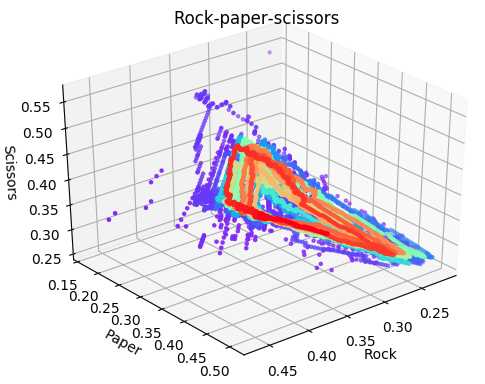
\includegraphics[scale=0.37]{figure/thirdGameSecondPolicy1m.png}
\caption{Policy convergence trajectory of player 1 head versus player 2 head. Start point $(0.10, 1)$, end point $(0.59, 0.50)$}
\label{Fig:thirdPolSecondGame11}
\end{figure}

\begin{figure}[!t]

\centering
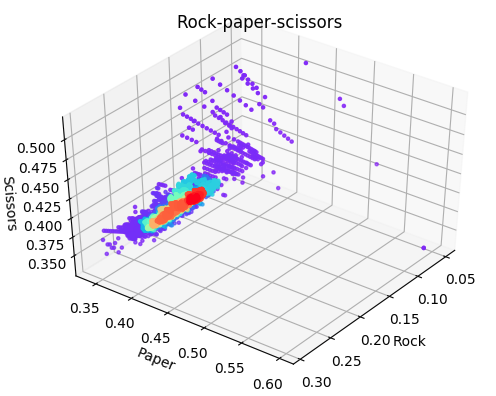
\includegraphics[scale=0.37]{figure/thirdGameSecondPolicy2m.png}
\caption{Policy convergence trajectory of player 1 head versus player 2 head. Start point $(0.20, 0.56)$, end point $(0.50, 0.55)$}
\label{Fig:thirdPolSecondGame12}
\end{figure}

(c) The modified algorithm works better for rock-paper-scissors, approaches $(1/3, 1/3, 1/3)$ point, and wanders around it nevertheless does not meet it \cite{the} (shown in Figure \ref{Fig:thirdPolSecondGame11} and \ref{Fig:thirdPolSecondGame12}).

(d) The policy is both a Nash equilibrium and a Pareto optimal because it has the maximum entropy possible.

(e) The value of the game is typically between $-0.1$ and $0.1$ since this game is a zero-sum game (fair game) which implies that expectation of reward is 0 for both.

(f) The added term hampers the bounce of policy value and directs it toward expected value.

\section{Notes About the Code}

There are 12 files of code, 6 of them are the main code, and the others serve as a function file for the main. The names of the files are chosen appropriately, such that they totally indicate for which part of the assignment they are. Codes are written in Python 3.6.8 with standard libraries, namely, Numpy and Matplotlib. The VS code is used as the editor of the code.

\bibliography{ref.bib}
\bibliographystyle{IEEEtran}

\end{document}